% !TeX root = ../Notizen.tex

\section*{Aufgabe 4: Kepler-Ellipsen}
Das Programm aus Aufgabe 1 wird jetzt verwendet um die Planeten Bahnen zu bestimmen.
Dazu wird die Zentralkraft verwenden
\begin{align}
	\frac{1}{m}\vec{F}(\vec{r})=-G\frac{\vec{r}}{r^3}
\end{align}
Wobei $G=1$ gesetzt wurde.
\subsection*{a)}
Hier werden zwei Teilchen Bahnen für die Masse = $1kg$ erstellt.
Für das erste Teilchen werden die Startvektoren 
\begin{align}
	\vec{r}_1=
	\begin{pmatrix}
		1,0\\0,0\\0,0
	\end{pmatrix}\text{ und }
	\vec{v}_1=
	\begin{pmatrix}
		-0,5\\1,0\\0,0
	\end{pmatrix}
\end{align}
verwendet und für den zweiten
\begin{align}
	\vec{r}_2=
	\begin{pmatrix}
		1,0\\0,0\\0,0
	\end{pmatrix}\text{ und }
	\vec{v}_2=
	\begin{pmatrix}
		-0,1\\1,0\\0,0
	\end{pmatrix}.
\end{align}
Die Resultierenden Bahnen sind in \cref{fig:Bahn} dargestellt.
Diese wurden mit $h=0.01$ und $t=10$ erstellt.
In \cref{fig:Bahn2} ist die Bahn für größere Breiten dargestellt. ist lässt sich erkennen das die Ellipse erst eckiger wird und später wie eine Spirale zum Ursprung bewegt.
Für kleine Anfangsgeschwindigkeiten, fällt das Teilchen in den Ursprung und bekommt eine starke Beschleunigung und läuft dann weg, wie in \cref{fig:Bahn3} dargestellt.\\

\begin{figure}[h!]
	\begin{subfigure}[c]{0.5\textwidth}
		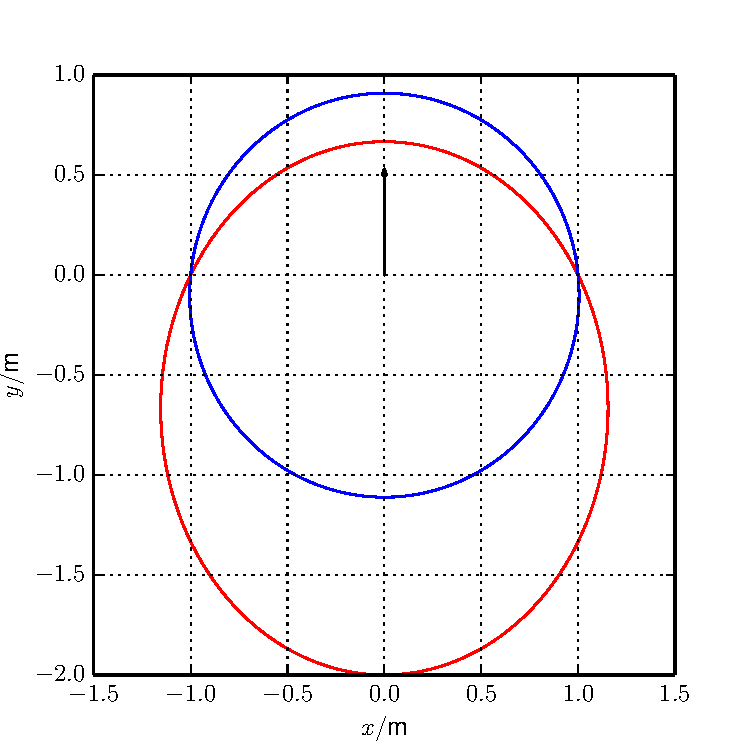
\includegraphics[width = \textwidth]{../Plots/Plot_4_A_1.pdf}
		\caption{Hier sind die 2 Simulierten Planeten Bahnen dargestellt, sowie der Lenz-Runge-Vektor.\label{fig:Bahn}}
	\end{subfigure}
	\begin{subfigure}[c]{0.5\textwidth}
		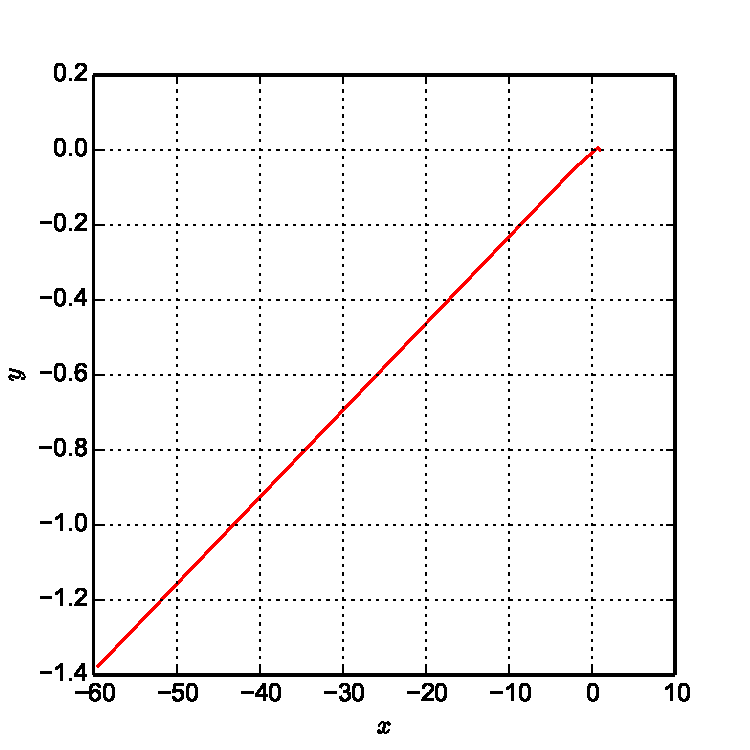
\includegraphics[width = \textwidth]{../Plots/Plot_4_A_5.pdf}
		\caption{ Hier ist dargestellt wie sich die Bahn für kleine Anfangsgeschwindigkeiten verhält. \label{fig:Bahn3}}
	\end{subfigure}
	\begin{subfigure}[c]{0.5\textwidth}
		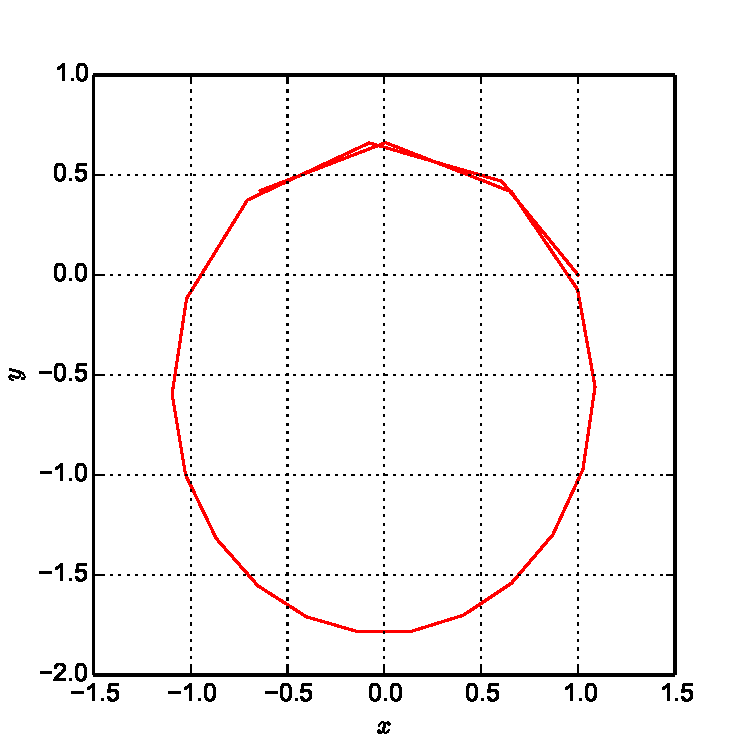
\includegraphics[width = \textwidth]{../Plots/Plot_4_A_3.pdf}
		\caption{ Hier sind die Bahnen für $h=0,5$ dargestellt.}
	\end{subfigure}
	\begin{subfigure}[c]{0.5\textwidth}	
		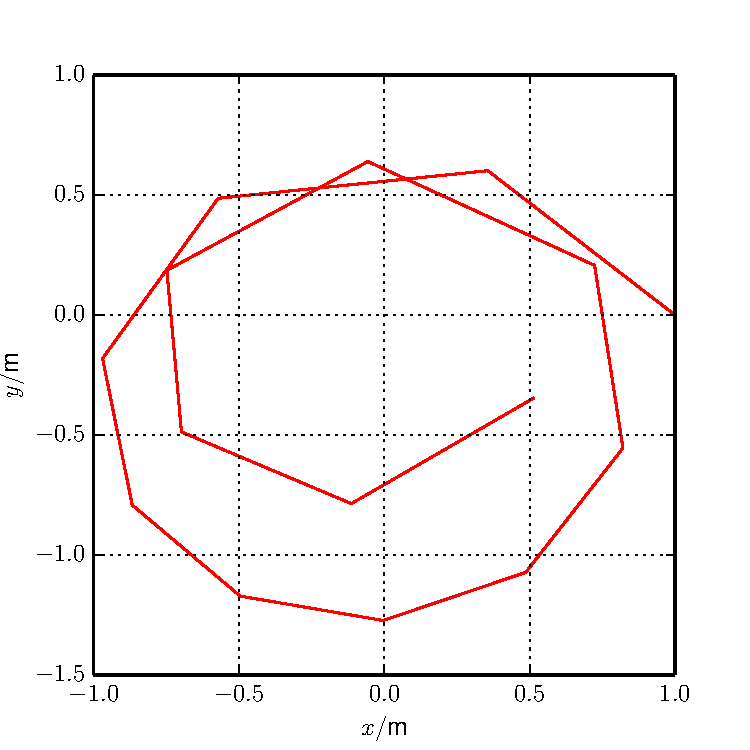
\includegraphics[width = \textwidth]{../Plots/Plot_4_A_4.pdf}
		\caption{ Hier sind die Bahnen für $h=0,7$ dargestellt.\label{fig:Bahn2}}
	\end{subfigure}\\
\end{figure}
\subsection*{b)}
Als nächstes soll überprüft werden ob die Energie in dem System erhalten ist.
Dabei ist die Energie definiert als
\begin{align}
	E=\frac{1}{2}v^2-\frac{mG}{r}
\end{align}
Hier wird wieder 
